\documentclass[12pt, titlepage]{article}

\usepackage{booktabs}
\usepackage{tabularx}
\usepackage{hyperref}
\usepackage{float}
\usepackage{graphicx}
\usepackage{color}
\usepackage{soul}
\usepackage[shortlabels]{enumitem}
\hypersetup{
    colorlinks,
    citecolor=black,
    filecolor=black,
    linkcolor=blue,
    urlcolor=blue
}
\usepackage[round]{natbib}

\title{SE 3XA3: Software Requirements Specification}

\author{Group \#10
        \\Lab: L03
		\\ Aamina Hussain, hussaa54
		\\ Jessica Dawson, dawsor1
		\\ Fady Morcos, morcof2
}

\date{}

%\input{../Comments}

\begin{document}

\maketitle

\pagenumbering{roman}
\tableofcontents
\listoftables
\listoffigures

\begin{table}[h!]
\caption{\bf Revision History}
\begin{tabularx}{\textwidth}{p{3cm}p{2cm}X}
\toprule {\bf Date} & {\bf Version} & {\bf Notes}\\
\midrule
Feb 9, 2022 & 0.0 & Initial Document; Completed Section 1, 2.1.1, 3.1, 3.2\\
Feb 11, 2022 & 0.1 & Completed Section 2.1.2, 2.1.3, 2.2, 3.3-3.9, 4, 5\\
\color{red}Apr 11, 2022 & \color{red}1.0 & \color{red}Updated FRs, Added Fit Criterion for NFRs\\
\bottomrule
\end{tabularx}
\end{table}

\clearpage


\pagenumbering{arabic}

This document describes the requirements for the Abstract Art Generator. The template for the Software
Requirements Specification (SRS) is a subset of the Volere template.%~\citep{RobertsonAndRobertson2012}.

\section{Project Drivers}

\subsection{The Purpose of the Project}

The purpose of the proposed project is to enhance an existing art generator. The existing Abstract Art Generator can create a wide array of different images with many customization options. The project will add to these options by increasing the ways the art can be generated and manipulated. The finished product should allow for even more variation in art generation.

\subsection{The Stakeholders}

\subsubsection{The Client}

The project's clients will be Dr. Asghar Bokhari as the instructor of SFWRENG 3XA3 and the TAs of the course. They are interested in expanding the Abstract Art Generator and will be determining whether the requirements have been met.

\subsubsection{The Customers}

The customers of the project are all those who are interested in generating abstract art. 

\subsubsection{Other Stakeholders}

The developers of the project are also stakeholders as they will be applying their skills to the project. The developer of the original Abstract Art Generator, Burak Unutmaz, is also a stakeholder as they have an interest in seeing how their project expands.

\subsection{Mandated Constraints}

\begin{enumerate}
    \item The project must run on Windows 10 or newer, or Linux Ubuntu 20.04.
    \item The project must be completed according to the schedule included in Tasks (Section 4.4).
\end{enumerate}

\subsection{Naming Conventions and Terminology}

\begin{itemize}
    \item \textbf{Color Palette}: Up to eight different colors that complement each other that the generated abstract art is made up of.
    \item \textbf{Layer}: The Abstract Art Generator contains layers. Each layer is made up of a specified shape laid out in a specified pattern. The colors of these shapes are from the chosen color palette. The layers are then stacked on top of each other to create the finished art piece.
\end{itemize}

\subsection{Relevant Facts and Assumptions}

\subsubsection{Facts}

\begin{itemize}
    \item N/A
\end{itemize}

\subsubsection{Assumptions}

\begin{itemize}
    \item Users have access to a computer
    \item Users know how to use a computer
    \item Users know how to download files
    \item Users can read English
\end{itemize}

\section{Functional Requirements}

\subsection{The Scope of the Work and the Product}

\subsubsection{The Context of the Work}

\begin{figure}[H]
    \centering
    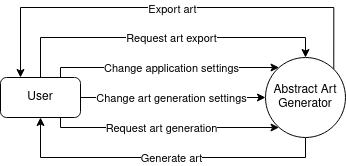
\includegraphics[width=0.55\textwidth]{context diagram.png}
    \caption{Work Context Diagram}
    \label{fig:context}
\end{figure}

\subsubsection{Work Partitioning}

\begin{table}[H]
    \centering
    \begin{tabular}{|c|l|c|l|} \hline
        \textbf{Event Number} & \textbf{Event Name} & \textbf{Input} & \textbf{Output} \\ \hline
        1 & Generating a picture & Mouse & Generated Picture \\ \hline
        2 & Exporting a picture & Keyboard/Mouse & Image File \\ \hline
        3 & Opening the help overlay & Mouse & Help Overlay \\ \hline
        3 & Opening the settings menu & Mouse & Settings Menu \\ \hline
    \end{tabular}
    \caption{Work Partitioning Events}
    \label{tab:WorkPart1}
\end{table}

\begin{table}[H]
    \centering
    \begin{tabular}{|c|p{120mm}|} \hline
        \textbf{Event Number} & \textbf{Summary} \\ \hline
        1 & The user can, through mouse input, choose to manipulate and change generation settings and generate an image. The image will then be displayed to the user in the UI. \\ \hline
        2 & The user, through mouse and keyboard input, can specify a resolution and file location to export an image file to. \\ \hline
        3 & The user can open and read the help menu by using mouse input \\ \hline
        3 & The user can open and manipulate the applications' setting by using mouse input \\ \hline
    \end{tabular}
    \caption{Work Partitioning Summaries}
    \label{tab:WorkPart2}
\end{table}

\subsubsection{Individual Product Use Cases}

\begin{figure}[H]
    \centering
    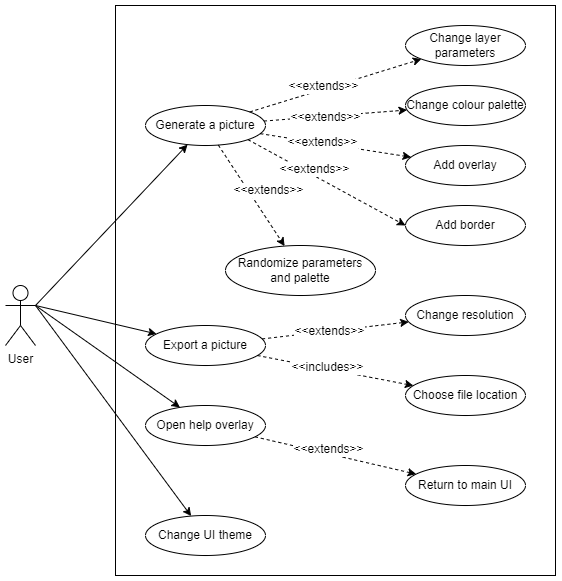
\includegraphics[width=0.8\textwidth]{UseCasesUpdated.png}
    \caption{Use Case Diagram}
    \label{fig:context}
\end{figure}

The above diagram specifies the product use cases. Generating a picture is the most complex as it involves changing generation parameters. Exporting a picture requires a resolution and file location to be specified. Opening the help overlay and changing the UI theme just involves the user accessing a \texttt{HELP} button or \texttt{THEME} button.
% Opening the settings menu allows the user to change aspects of the UI and program itself.

\subsection{Functional Requirements}
FR1. The system shall have at least 30 unique color palette options.
\begin{itemize}
    \item Rationale: The user will have a wider range of color options to choose from.
\end{itemize}
FR2. The system shall allow the user to choose the background color of the art from the chosen color palette.
\begin{itemize}
    \item Rationale: The user may want to choose the exact background color instead of it being randomly chosen from the color palette.
\end{itemize}
FR3. The system shall display which color the user chose as the background.\\
\\
FR4. The system shall allow the user to have three generated layers.
\begin{itemize}
    \item Rationale: Currently, the program only allows for two generated layers. This will increase the variety of art the user can generate.
\end{itemize}
FR5. The system shall allow the user to change the transparency of the layers.
\begin{itemize}
    \item Rationale: This will increase the variety of art the user can generate.
\end{itemize}
FR6. The system shall allow the user to have text on top of the art.
\begin{itemize}
    \item Rationale: This will increase the variety of art the user can generate.
\end{itemize}
FR7. The system shall allow the user to change the font of the text on top of the art.\\
\\
FR8. The system shall allow the user to change the size of the text on top of the art.\\
\\
\st{FR9. The system shall allow the user to change the color of the text on top of the art.}\\
\color{red} \#\#COMMENT: We decided to not implement this requirement and allow the color of the text to be randomly chosen from the color palette of the current generated art image. This is because in order to allow the user to choose the text color, we would need to include a long list of colors, and it is likely that most colors would clash with the generated art. The art will look more cohesive using a color from the current color palette. \color{black}\\
\\
FR9. The system shall allow the user to add a border to the art.
\begin{itemize}
    \item Rationale: This will increase the variety of art the user can generate.
\end{itemize}
FR10. The system shall display the border options.\\
\\
\color{red}FR11. The system shall display the instructions for using the program.
\begin{itemize}
    \item Rationale: This will promote the system's usability.
\end{itemize}\color{black}
\st{FR12. The system shall display the display settings.}\\
\\
FR12. The system shall allow the user to switch between different UI themes, such as dark mode and light mode.
\begin{itemize}
    \item Rationale: This will increase accessibility and allow users to adjust the UI theme to their comfort level.
\end{itemize}

\section{Non-functional Requirements}

\subsection{Look and Feel Requirements}

\subsubsection{Appearance Requirements}
LF1. The menu of the program must be formatted neatly and not be cluttered.
\begin{itemize}
    \item Rationale: The user should find the appearance of the program menu attractive to further their interest in using the program.
    \item \color{red} Fit Criterion: The different sections of the menu will be in-line with each other and have the same width. \color{black}
\end{itemize}
\subsubsection{Style Requirements}
LF2. The program background must be a simple and solid color.
\begin{itemize}
    \item Rationale: If the program background is not simple, it may clash with the generated art and end up distracting the user.
    \item \color{red} Fit Criterion: The program background will be one single color. \color{black}
\end{itemize}

\subsection{Usability and Humanity Requirements}
\subsubsection{Ease-Of-Use Requirements}
UH1. The options of the program shall be easy for the user to access via the program menu.
\begin{itemize}
    \item Rationale: The user should be able to select any option efficiently and should not struggle to find the options.
    \item \color{red} Fit Criterion: All of the program options will be reasonably sized, positioned, and displayed on the program menu. \color{black}
\end{itemize}
\subsubsection{Accessibility Requirements}
UH2. The UI text shall be legible for the average user.
\begin{itemize}
    \item Rationale: The average user cannot make full use of the features if they find it difficult to read the instructions or option descriptions.
    \item \color{red} Fit Criterion: The UI text size will be 12 pt. \color{black}
\end{itemize}
\subsubsection{Learning Requirements}
UH3. The instructions for the program shall be clearly available to the user via the program menu.
\begin{itemize}
    \item Rationale: The instructions are necessary for the user to be able to use the program.
    \item \color{red} Fit Criterion: All of the program instructions can be accessed by the user through a \texttt{HELP} option in the program menu. \color{black}
\end{itemize}
\subsection{Performance Requirements}
\subsubsection{Speed and Latency Requirements}
PR1. The system shall respond to the user's parameter input or selection within a reasonable time frame.
\begin{itemize}
    \item Rationale: The user will not appreciate having to wait too long for the system to respond to their change.
    \item \color{red} Fit Criterion: The system's response time to the user's input should be no longer than MAX\_PARAM\_TIME. \color{black}
\end{itemize}
PR2. The system shall generate an image within a reasonable time frame.
\begin{itemize}
    \item Rationale: The user will not appreciate having to wait too long for the system to respond to their change.
    \item \color{red} Fit Criterion: The time taken for the system to generate an image should be no longer than MAX\_GENERATION\_TIME. \color{black}
\end{itemize}
\subsubsection{Reliability and Availability Requirements}
PR3. The program shall be available for the user to run whenever they wish.
\begin{itemize}
    \item Rationale: The program does not require any external resources since it is downloaded and run on the user's machine. So the program should be designed such that as long as the user's PC is working, they should be able to run the program.
    \item \color{red} Fit Criterion: The program launches 99\% of the time when the user's PC is functional. \color{black}
\end{itemize}

\subsection{Operational and Environmental Requirements}
\subsubsection{System Requirements}
OE1. The program shall be able to run on most moderm operating systems.
\begin{itemize}
    \item Rationale: The program should be available to user's with common operating systems.
    \item \color{red} Fit Criterion: The program shall be able to run on Windows 10 or newer, or Linux Ubuntu 20.04. \color{black}
\end{itemize}

\subsubsection{Productization Requirements}
OE2. The program shall be available as an executable file for the user to download.
\begin{itemize}
    \item Rationale: Having the program like this will ensure it is not difficult for the user to install.
\end{itemize}

\subsection{Maintainability and Support Requirements}
\subsubsection{Maintenance Requirements}
MS1. The source code shall be fully documented and consistent.
\begin{itemize}
    \item Rationale: This will make it simpler and more straightforward for the current and future developers to understand.
    \item \color{red} Fit Criterion: The source code shall be fully documented using doxygen comments. \color{black}
\end{itemize}
\subsubsection{Support Requirements}
MS2. The program's repository will be public.
\begin{itemize}
    \item Rationale: A public repository for the program will allow users to raise issues and access the most updated information regarding the program's development.
\end{itemize}

\subsection{Security Requirements}
N/A
\subsection{Cultural and Political Requirements}
CP1. The program instructions or feature descriptions shall not have any culturally offensive or politically sensitive words, phrases, or symbols.


\subsection{Legal Requirements}
LR1. The program shall adhere to and not violate any Canadian or US laws.

\subsection{Health and Safety Requirements}
N/A

\section{Project Issues}

\subsection{Open Issues}

\begin{enumerate}[start=1,label={Issue \arabic*.}]
    \item Currently all the code for the original Abstract Art Generator program is written and contained within one single module composed of 1400 lines of code. This creates an issue for understandability and maintainability. Having poor modularity makes future adjustments and modification difficult. The next developer to try and update or make adjustments to the program may run into trouble comprehending it and thus have a hard time altering the program. 
\end{enumerate}

\subsection{Off-the-Shelf Solutions}

There are many websites and applications which also generate random art similar to what our project does (for example, \href{https://www.randomart.co.uk/random-art-generator.aspx}{randomart.co.uk}). However, there are not many open-source random art generators, and it is unlikely we will be using any other sources of code. Most of the adapted code will be coming from the original Abstract Art Generator we are enhancing.

\subsection{New Problems}

N/A

\subsection{Tasks}

\begin{enumerate}
    \item Begin modularizing the code.
    \item Add additional layers (allow for more than two generated art layers).
    \item Conduct first code review and debugging.
    \item Add text overlay feature to the abstract art generator.
    \item Add feature that allows user to set preferred background colour.
    \item \color{red} Add more color palette options.\color{black}
    \item \color{red} Change color palette implementation to allow color palettes of various lengths.\color{black}
    \item Conduct second code review and debugging.
    \item Add feature that allows user to change the UI theme.
    \item Conduct testing of the code.
    \item Conduct third code review and debugging.
    \item Conduct an analysis of the program against the functional and non-functional requirements.
\end{enumerate}

For a more detailed overview refer to the project \href{https://gitlab.cas.mcmaster.ca/3xa3-l3-g10/3xa3-l3-g10/-/tree/main/ProjectSchedule}{Gantt Chart}

\subsection{Migration to the New Product}

N/A. The new product will be a standalone version of the original Abstract Art Generator.
%As we get closer to the new version of the project, we will be incrementally adding and testing the new features. The program should have better migration, understandability and more customization features.

\subsection{Risks}

There is minimal risk associated with this project since it is an independent program that does not rely on any external resources. The one main risk is that since the code was not well managed originally, it may be difficult to understand and work with. This could cause delays and difficulty modifying the program. 

\subsection{Costs}

There is no monetary cost related to this project. This is because we are working on an open sourced project and the tools we are using are all free of cost. The only cost associated with this project is the time and effort our team will be spending on brainstorming, development, and testing, which is roughly 5-8 hours weekly for each team member.

\subsection{User Documentation and Training}

The program will include a help tab that the user can select to access the instructions. The GUI will be kept clean and simple so the user should not have any issue navigating the program menu.

\subsection{Waiting Room}

Possible future features to be added:

\begin{enumerate}
    \item Create a more appealing GUI (i.e. better choice of fonts, more attractive front-end, etc.).
    \item Add layer effects like distortion and noise.
    \item Add a feature that allows the program to design and generate 3-dimensional abstract art pieces.
    \item \color{red} Change the overlay/border section to have a scrolling dialogue box, which will allow more overlay and border options to be displayed.
    \item \color{red} Add an option to allow the user to change the size of the UI text.
\end{enumerate}

\subsection{Ideas for Solutions}

\begin{enumerate}[start=1,label={Issue \arabic*.}]
    \item A restructuring of the code may help in modularizing it to allow for better understandability, maintainability, and modification.
\end{enumerate}

\bibliographystyle{plainnat}

\bibliography{SRS}

\newpage

\section{Appendix}

N/A

\subsection{Symbolic Parameters}

\noindent MAX\_PARAM\_TIME: 1 sec

\noindent MAX\_GENERATION\_TIME: 10 sec

\end{document}
